\documentclass[10pt,a4paper]{article}
\usepackage{iftex}
\ifPDFTeX
  \usepackage[T2A]{fontenc}
  \usepackage[utf8]{inputenc}
\else
  \usepackage{fontspec}
  \setmainfont[BoldFont=cmunbx.otf,ItalicFont=cmunti.otf]{cmunrm.otf}
  \setmonofont{cmuntt.otf}
\fi
\usepackage[russian]{babel}
\usepackage[margin=16mm]{geometry}
\usepackage{graphicx,booktabs,tabularx,array,fancyvrb,amsmath,xcolor}
\usepackage[breaklinks=true,hidelinks]{hyperref}
\hypersetup{pdftitle={ДЗ5. Kubernetes: управление ресурсами и планирование},pdfauthor={Вдовина Анастасия Романовна}}
\setlength{\parindent}{0pt}
\setlength{\parskip}{5pt}
\setlength{\emergencystretch}{3em}
\renewcommand{\arraystretch}{1.13}
\newcolumntype{Y}{>{\raggedright\arraybackslash}X}
\raggedbottom
\newcommand{\MemoryPeak}{83.23}
\newcommand{\LimitMiB}{112}
\newcommand{\TunedRSS}{64.52}
\newcommand{\TunedCgroup}{56.36}
\newcommand{\CPUAlloc}{12000}
\newcommand{\CPUUsed}{1200}
\newcommand{\BlockingCPU}{9800m}
\newcommand{\LowCPU}{9800m}
\newcommand{\VerificationCount}{20}
\newcommand{\ProfileRows}{1 & 64.43 & 83.23 & 4.098 \\
2 & 64.57 & 56.27 & 3.970 \\
3 & 64.58 & 56.20 & 3.954 \\}
\newcommand{\ShardRows}{0 & 57347 & 694 & 210424605 & 1.337 \\
1 & 57347 & 804 & 210224414 & 1.340 \\
2 & 57347 & 820 & 212035661 & 1.389 \\
3 & 57347 & 805 & 215164762 & 1.395 \\}
\newcommand{\TopRows}{1 & go & postgresql & 1074 & 1074 \\
2 & docker & go & 696 & 696 \\
3 & go & sql & 545 & 545 \\
4 & git & go & 534 & 534 \\
5 & go & linux & 488 & 488 \\
6 & docker & postgresql & 464 & 464 \\
7 & go & kafka & 438 & 438 \\
8 & go & kubernetes & 411 & 411 \\
9 & go & python & 407 & 407 \\
10 & go & redis & 394 & 394 \\}

\begin{document}
\section*{ДЗ5. Kubernetes: управление ресурсами и планирование}
Вдовина Анастасия Романовна, ИИИ-3-ИнжДан-1-3.\newline
Вариант 7: «Программист, разработчик на Go». 26.11.2026.

\subsection*{1. Подготовка кластера и образа}
Подняла отдельный локальный кластер \texttt{de-hw5} через kind 0.27.0 в Docker
Desktop на macOS ARM64. В кластере один узел \texttt{de-hw5-control-plane},
на нём работают и управляющие компоненты, и учебные задания.
Kubernetes и kubectl --- 1.32.2, containerd --- 2.0.2.
Для воспроизводимости зафиксировала digest образа узла в \path{manifests/kind.yaml}.
Конфигурацию доступа сохранила отдельно в \path{work/kubeconfig}.

\begin{Verbatim}[fontsize=\small]
kind create cluster --name de-hw5 --config manifests/kind.yaml \
  --kubeconfig work/kubeconfig --wait 180s
docker build -t de-hw5-skills:1 .
kind load docker-image de-hw5-skills:1 --name de-hw5
kubectl get nodes
de-hw5-control-plane   Ready   control-plane   v1.32.2
\end{Verbatim}

Взяла \texttt{common.py} и \texttt{mapreduce.py} из своего ДЗ3, коммит
\texttt{795746ef9d0625748e467254bb45859eb3eab978}. Их содержимое совпадает
с репозиторием побайтно; проверка Git blob и SHA-256 --- в
\path{evidence/hw3-provenance.json}. Оболочка ДЗ5 вызывает прежние
\texttt{csv\_chunks} и \texttt{map\_chunk}, накапливает пары и сохраняет результат в S3.
Map по-прежнему формирует сочетания для $k=1,2,3$; в этом ДЗ публикую $k=2$.

Образ собрала на Python 3.12.8 с фиксированными зависимостями boto3.
Процесс запускается от UID 10001; в Job отключены токен ServiceAccount,
дополнительные capabilities и запись в корневую файловую систему.
Датасет и ключи S3 в образ не включены.

\subsection*{2. RustFS и исходные данные внутри Kubernetes}
Перенесла S3-хранилище из ДЗ2 в Deployment RustFS 1.0.1, сохранив схему
EC 2+2 и четыре каталога-диска. Каждому каталогу выделила отдельный PVC по
2 GiB; все четыре PVC получили статус Bound. Service \texttt{rustfs} даёт
доступ к S3 на 9000 и консоли на 9001. Задания используют внутренний DNS
\path{rustfs.hw5.svc.cluster.local:9000}, ключи получают из Secret.
Для загрузки с компьютера использовала локальный port-forward на 19000.

Загрузила в \texttt{hh-lake} исходный \texttt{raw/it\_vacancies\_2024.csv}:
847\,619\,384 байта, 229\,388 записей, 23 колонки.
После GET размер и SHA-256 совпали с ДЗ2 и ДЗ3:
\begin{Verbatim}[fontsize=\scriptsize]
303db922b541e4440906f5a7e8be32fb55e8808f950ffddb8c272f1548212a65
\end{Verbatim}
Также загрузила четыре части файла и прочитала каждую обратно.
Размеры и контрольные суммы записала в \path{evidence/source-upload.json}.
Это перенос сервиса, конфигурации EC и исходных данных в новые тома;
старые папки-диски ДЗ2 не изменяла. PVC находятся на одном компьютере,
поэтому этот стенд не защищает от отказа физического SSD.

\clearpage
\section*{Хранилище в консоли RustFS}
Скриншоты сняла в работающей консоли RustFS после загрузки данных.
В свойствах исходника виден полный размер файла; в каталоге parts лежат
четыре части CSV и их манифест.
\begin{center}
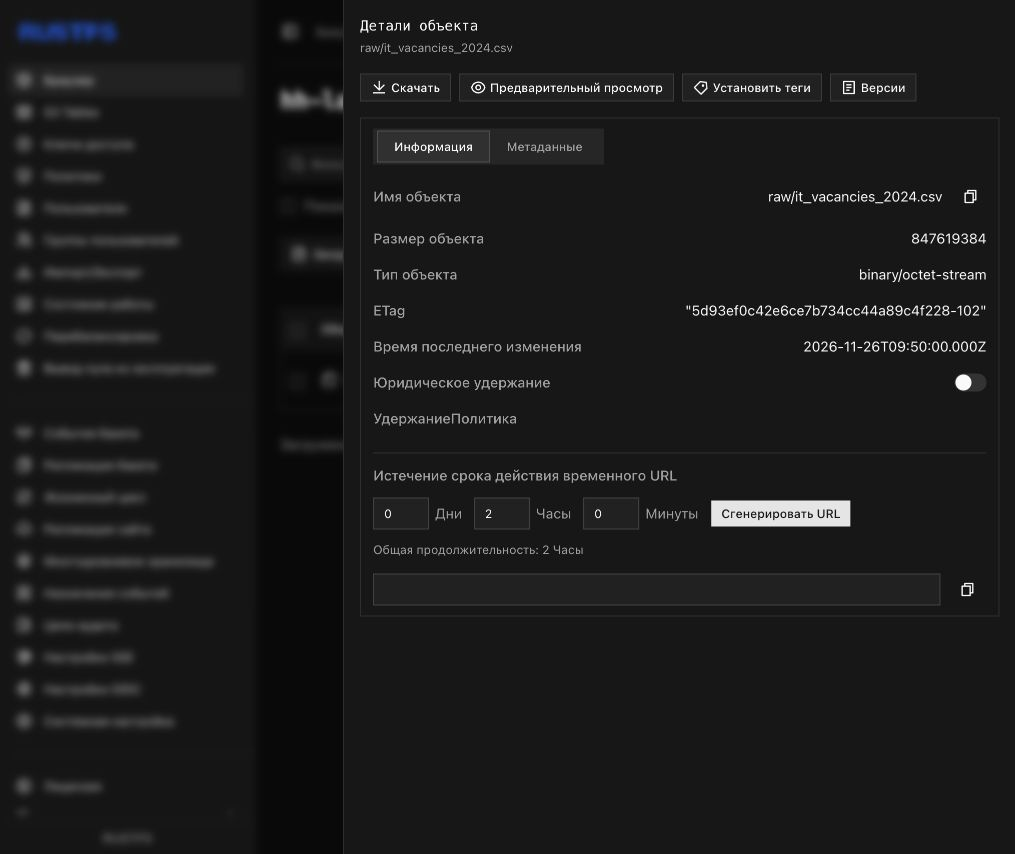
\includegraphics[width=\linewidth,trim=0 445 0 0,clip]{images/01-rustfs-source.png}
\par\smallskip{\footnotesize Рис. 1. Свойства исходного CSV: 847\,619\,384 байта.}
\end{center}
\begin{center}
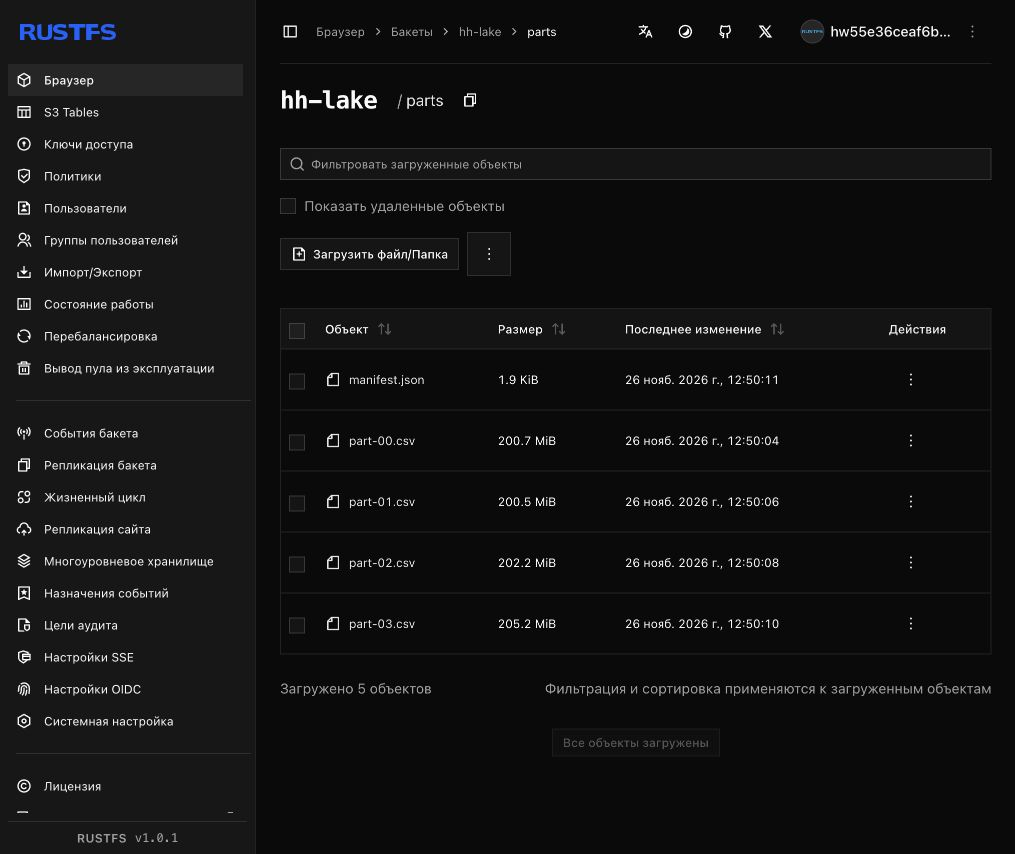
\includegraphics[width=\linewidth]{images/02-rustfs-parts.png}
\par\smallskip{\footnotesize Рис. 2. Четыре части файла в бакете hh-lake.}
\end{center}

\clearpage
\section*{3. Остановка по памяти и выбор предела}
Для одного и того же расчёта полного файла выполнила три измерения с
\texttt{requests: cpu=250m, memory=64Mi} и
\texttt{limits: cpu=1, memory=256Mi}. Файл читался из S3 потоком с буфером
1 MiB, чанками по 2\,000 записей. Каждый запуск завершился и дал все
частоты пар из ДЗ3 без расхождений.

\begin{center}
\begin{tabular}{rrrr}
\toprule
Запуск & Пик RSS, MiB & Пик cgroup, MiB & Расчёт, с \\
\midrule
\ProfileRows
\bottomrule
\end{tabular}
\end{center}
RSS получила из Linux \texttt{getrusage(RUSAGE\_SELF).ru\_maxrss}
с переводом KiB в байты. Полный пик контейнера прочитала из cgroup v2
\path{/sys/fs/cgroup/memory.peak}. В журналах также есть
\texttt{memory.max} и \texttt{memory.events}; пик включает сериализацию
результата и первый PUT в S3. Metrics Server для этих измерений не нужен.

\subsection*{Намеренно малый предел}
Снизила предел до 48 MiB, запрос памяти --- до 32 MiB.
Использовала тот же образ, полный CSV и код вычисления; искусственного
выделения памяти в программе нет. Получила \texttt{OOMKilled}, код 137:
\begin{Verbatim}[fontsize=\scriptsize]
pod=skills-oom-mw9nn
requests.memory=32Mi  limits.memory=48Mi
reason=OOMKilled  exitCode=137
startedAt=2026-11-26T09:50:34Z  finishedAt=2026-11-26T09:50:39Z
\end{Verbatim}

В Job задала \texttt{restartPolicy: Never} и \texttt{backoffLimit: 0}.
Поэтому остановленный контейнер остался доступен для проверки и не был
скрыт автоматическим успешным повтором. Доказательство ---
\path{evidence/skills-oom-pods.json} и соответствующий журнал контейнера.

\subsection*{Расчёт рабочего предела}
Взяла наибольшее значение RSS и cgroup среди трёх запусков:
$P=\MemoryPeak$ MiB. Добавила 25\% и округлила вверх до кратного 16 MiB:
\[
L=16\cdot\left\lceil\frac{1.25P}{16}\right\rceil
 = \LimitMiB\ \text{MiB}.
\]
Повторила полный расчёт с \texttt{requests.memory=64Mi} и
\texttt{limits.memory=\LimitMiB Mi}. Job \texttt{skills-tuned} завершился;
пик RSS --- \TunedRSS\ MiB, cgroup --- \TunedCgroup\ MiB,
\texttt{oom\_kill=0}, все частоты совпали с эталоном.
Числа, формула и Kubernetes status сохранены в
\path{evidence/memory-summary.json}.

Запрос памяти нужен планировщику для размещения; он не задаёт предел
процессу. Предел памяти контролирует ядро через cgroup, превышение может
привести к OOM kill. Предел CPU ограничивает время процессора и обычно
вызывает throttling, а не OOMKilled.

\clearpage
\section*{4. Параллельный расчёт по частям файла}
Разбила CSV штатным парсером на четыре последовательных диапазона по
57\,347 записей. Внутри описаний вакансий есть переводы строк в кавычках,
поэтому деление по физическим строкам или произвольным байтам здесь
повредило бы записи. В каждой части сохранила все 23 колонки и заголовок.
Части вместе покрывают записи $[0;229388)$ без пересечений.
Хеш последовательности записей до и после разбиения совпал по всем
полям и порядку; проверка --- \path{evidence/partition-record-integrity.json}.

Создала Indexed Job: \texttt{completions=4}, \texttt{parallelism=4}.
Индекс \texttt{JOB\_COMPLETION\_INDEX} определяет объект
\texttt{parts/part-00.csv}--\texttt{part-03.csv}. Каждый Pod читает свою
часть из RustFS и пишет полные счётчики в отдельный объект
\texttt{runs/parallel/part-NN.json}. Всем работникам задала запрос
250m CPU / 64 MiB и предел 1 CPU / \LimitMiB\ MiB.

\begin{center}
\begin{tabular}{rrrrr}
\toprule
Индекс & Записей & Вариант Go & Размер CSV, байт & Расчёт, с \\
\midrule
\ShardRows
\bottomrule
\end{tabular}
\end{center}
У всех четырёх контейнеров интервалы исполнения пересекаются;
\texttt{completedIndexes=0-3}. После завершения отдельный Job
\texttt{skills-reducer} прочитал четыре результата, проверил ровно один
результат на каждый индекс и сложил частоты одинаковых пар.
Повтор работника перезаписывает объект его индекса; reducer не складывает
результаты разных попыток одного индекса. Из каждой части передаю все
пары: объединение только локальных топ-10 могло бы потерять глобально
частую пару.

Фильтр остался прежним: роль «Программист, разработчик» и Go/Golang
отдельным словом в названии либо точным навыком. Пробелы и дубли навыков
удаляются, регистр приводится к нижнему, Golang объединяется с Go.
Получила 3\,123 вакансии, 13\,552 различные пары и 61\,694 вхождения пар.

\begin{center}
\begin{tabular}{rllrr}
\toprule
№ & Навык 1 & Навык 2 & ДЗ3 & Kubernetes \\
\midrule
\TopRows
\bottomrule
\end{tabular}
\end{center}
Сравнила не только топ-10, но и все 13\,552 ключа с каждой частотой:
\texttt{baseline\_equal=true}, расхождений 0. Эталон взят из того же коммита
ДЗ3. Итоговые файлы --- \path{results/counts_2.json},
\path{results/top10.json}; статусы и результаты частей ---
\path{evidence/parallel-summary.json}, \path{evidence/parallel-shards.json}.

\clearpage
\section*{5. Ожидание CPU и вытеснение}
\subsection*{Ожидание при нехватке CPU}
Узел сообщает \CPUAlloc\ millicpu allocatable.
Перед опытом сумма запросов работающих Pod во всех пространствах имён
составила \CPUUsed\ millicpu. Служебный Pod \texttt{cpu-reservation}
запросил ещё \BlockingCPU, оставив 1\,000 millicpu.
Он ожидает в \texttt{sleep}: опыт проверяет резервирование через requests,
а не загрузку CPU по показаниям монитора.

Задание \texttt{skills-cpu-wait} запросило 2\,000 millicpu и осталось
\texttt{Pending}. Планировщик указал \texttt{Insufficient cpu}:
\begin{Verbatim}[fontsize=\scriptsize]
pod=skills-cpu-wait-6mcbc  phase=Pending
PodScheduled=False  reason=Unschedulable
0/1 nodes are available: 1 Insufficient cpu. preemption: 0/1 nodes are available: 1 No preemption victims
  found for incoming pod.
\end{Verbatim}

У ожидающего Pod не было назначенного узла и запущенного контейнера.
Удаление \texttt{cpu-reservation} освободило запрос, после чего тот же Pod
был назначен и завершил расчёт. UID до и после ожидания совпал.
Снимки --- \path{evidence/cpu-pending.json} и
\path{evidence/skills-cpu-wait-pods.json}. Планировщик проверяет сумму
requests, а не мгновенный фактический расход CPU.

\subsection*{Вытеснение задания с низким приоритетом}
В PriorityClass задала значения 100 для \texttt{hw5-low} и 1000 для
\texttt{hw5-high}. Для высокого приоритета оставила политику
\texttt{PreemptLowerPriority}.
Низкоприоритетный Job \texttt{skills-low} запросил \LowCPU\ и циклически
выполнял реальный расчёт ДЗ3. Дождалась записи о прочитанном первом чанке.
Затем запустила \texttt{skills-high} с запросом 2 CPU.
Свободного CPU ему не хватало, и scheduler выбрал низкоприоритетный Pod
для вытеснения. RustFS имеет тот же высокий приоритет и жертвой этого
опыта не является.

\begin{Verbatim}[fontsize=\scriptsize]
victim=skills-low-rh7mj
uid=39cebae7-2c98-4df3-b4e7-21207a83632f
DisruptionTarget=True  reason=PreemptionByScheduler
Preempted by pod 3248e887-3950-4a2e-94eb-e88f1aeeeca4 on node de-hw5-control-plane
\end{Verbatim}

У жертвы зафиксировала условие \texttt{DisruptionTarget=True}, причину
\texttt{PreemptionByScheduler} и событие \texttt{Preempted}.
Обработчик SIGTERM оставляет 8 секунд на завершение, чтобы успеть сохранить
условие и UID удаляемого Pod. Высокоприоритетный Job получил узел и
завершил вычисление. Затем удалила низкоприоритетный Job, чтобы его
контроллер не продолжал создавать работников.

Это вытеснение планировщиком для освобождения запросов ресурсов.
Остановка по лимиту памяти в разделе 3 произошла внутри cgroup и имеет
другую причину. Высокий приоритет помогает только тогда, когда удаление
более низких Pod делает размещение возможным; он не добавляет ресурсов
узлу и не отменяет квоту. Полные свидетельства ---
\path{evidence/preemption-victim.json}, \path{evidence/preemption-events.json}
и \path{evidence/preemption-summary.json}.

\clearpage
\section*{6. Квота пространства имён}
В отдельном namespace \texttt{hw5-quota} создала ResourceQuota:
\begin{Verbatim}[fontsize=\small]
hard:
  requests.cpu: "1"
  requests.memory: 256Mi
  limits.cpu: "2"
  limits.memory: 512Mi
  pods: "4"
\end{Verbatim}
Первый Pod запросил 600m CPU / 64 MiB, пределы --- 600m CPU / 128 MiB.
Его создание прошло, квота показала использованные \texttt{requests.cpu=600m}.
Второй Pod с такими же ресурсами превысил бы квоту запросов CPU:
$600+600=1200>1000$ millicpu. API отклонил создание:
\begin{Verbatim}[fontsize=\scriptsize]
Error from server (Forbidden):
pods "quota-second" is forbidden: exceeded quota: compute-budget, requested: requests.cpu=600m, used:
  requests.cpu=600m, limited: requests.cpu=1
\end{Verbatim}

Второй Pod на этом этапе вообще не появился в API. Это отличается от
\texttt{Pending} в разделе 5, где объект Pod уже существовал, но scheduler
не мог выбрать узел. После удаления первого Pod и обновления
\texttt{status.used} до нуля повторила тот же запрос на создание второго:
он был принят и перешёл в \texttt{Running}. Сохранила квоту до и после
освобождения, текст отказа и принятый Pod в \path{evidence/quota-*}.
Квота ограничивает сумму заявок и пределов namespace; наличие свободного
CPU на узле не позволяет её обойти.

\subsection*{7. Проверка результата и состав репозитория}
Автотесты проверяют разбиение многострочного CSV, подсчёт пар при прежнем
фильтре, отсутствие повторного учёта индексов, порядок топ-10 при равных
частотах, расчёт предела памяти и учёт CPU всех пространств имён.
Отдельный \texttt{verify\_evidence.py} сверяет реальные Kubernetes status,
контрольные суммы, частоты и события. Все \VerificationCount\ проверок
доказательств прошли.

\begin{center}
\begin{tabularx}{\linewidth}{lX}
\toprule
Файлы & Содержание \\
\midrule
\texttt{Dockerfile, requirements*.txt} & Сборка образа и зависимости \\
\texttt{hw3/, baseline/} & Неизменённый расчёт и эталон ДЗ3 \\
\texttt{hw5/, scripts/} & Работник, reducer и воспроизводимые опыты \\
\texttt{manifests/} & kind, RustFS, PVC, Service, Jobs, приоритеты, квота \\
\texttt{evidence/} & Журналы команд, Pod/Job status, события, сверки \\
\texttt{results/} & Все частоты пар и совпадающий топ-10 \\
\texttt{report/} & Исходники этого отчёта в LaTeX \\
\bottomrule
\end{tabularx}
\end{center}

Репозиторий: \url{https://github.com/lilnacl/data-engineering-hw5-kubernetes}.
В README указала запуск с полного CSV, его ссылку и SHA-256.
Сам CSV, kubeconfig и действующие ключи S3 в репозиторий не включала.
Манифесты фактически выполненных Job находятся в \path{manifests/runs/}.
Узел и четыре тома локальные: проверены механизмы управления ресурсами,
а не отказоустойчивость нескольких физических машин.

\clearpage
\section*{8. Соответствие YARN, Mesos и Kubernetes}
В лекции YARN рассматривается как централизованная модель выделения
ресурсов, Mesos --- как двухуровневая. В своём стенде использовала
стандартный централизованный kube-scheduler. Ниже привела соответствия
по роли компонентов; полного совпадения объектов между системами нет.

\begin{center}
\small
\begin{tabularx}{\linewidth}{>{\raggedright\arraybackslash}p{24mm}YYY}
\toprule
Роль & YARN & Mesos & Kubernetes в работе \\
\midrule
Глобальное выделение ресурсов & ResourceManager и его scheduler & Master/allocator предлагает ресурсы framework & kube-scheduler выбирает узел для Pod \\
Исполнение на узле & NodeManager запускает контейнеры & Agent запускает executor, тот исполняет задачи & kubelet и containerd запускают контейнеры Pod \\
Координация приложения & Отдельный ApplicationMaster & Framework scheduler и executor & Job controller следит за Pod и повторами; worker/reducer выполняют алгоритм \\
Единица размещения & YARN container: выделенные CPU/RAM & Tasks используют ресурсы принятого offer & Pod с заявками ресурсов контейнеров \\
Способ запроса & AM запрашивает контейнеры у RM & Framework принимает/отклоняет offer & В Pod задаются requests, scheduler находит подходящий узел \\
Разделение между пользователями & Очереди Capacity/Fair Scheduler & Политика allocator, роли framework & Namespace и ResourceQuota; PriorityClass для очередности/вытеснения \\
\bottomrule
\end{tabularx}
\end{center}

\textbf{Кто соответствует ApplicationMaster?}
В этом примере его функции разделены: Job controller поддерживает нужное
число успешных работников и повторяет сбои, а мой код выбирает часть
данных и выполняет reduce. Универсального отдельного AM на каждый Job
Kubernetes не запускает. Job controller не знает семантику пар навыков;
я запускаю reducer после успешных четырёх индексов.

\textbf{Является ли YARN container Docker-контейнером?}
Это прежде всего выделение ресурсов и контекст запуска процесса.
Docker может быть одним из способов исполнения в YARN, но термин
container сам по себе не означает OCI-образ. В Kubernetes Pod --- единица
планирования и может содержать несколько контейнеров. Mesos executor
также не равен Pod: он может обслуживать несколько задач framework.

\textbf{Квота Kubernetes соответствует Capacity Scheduler?}
Частично: обе политики ограничивают потребление группы приложений.
Но ResourceQuota задаёт верхнюю границу namespace и отклоняет лишний Pod;
она не гарантирует долю физических CPU, не реализует эластичные очереди
и не обеспечивает DRF. Гарантии ёмкости очередей и заимствование свободной
доли требуют соответствующего планировщика. Namespace --- область
объектов и политики, а не выделенная машина.

\textbf{Как связаны приоритет и справедливость?}
PriorityClass позволяет предпочесть важный Pod и вытеснить менее важный,
как в моём опыте. Это не равное распределение долей между всеми
приложениями. DRF сравнивает доминирующую долю каждого участника по
нескольким ресурсам; стандартные PriorityClass и ResourceQuota такую
политику сами не задают.

\clearpage
\section*{9. Ответы на вопросы лекции}
\textbf{Зачем общий менеджер ресурсов вместо отдельных кластеров?}
Он позволяет использовать свободные ресурсы одного приложения для
другого. Например, у MapReduce занят CPU ночью, у Spark днём: два
изолированных кластера оставляли бы часть машин без работы. Общий пул
уменьшает этот простой, а очереди/приоритеты ограничивают взаимное влияние.
В моём кластере S3-сервис и вычислительные задания делят один узел.

\textbf{В чём разница централизованного и двухуровневого планирования?}
В YARN ResourceManager выделяет контейнеры по общей политике, а AM
координирует приложение. В Mesos allocator сначала решает, какому framework
предложить ресурсы; затем framework scheduler выбирает задачи и ресурсы
из offer. В обычном Kubernetes готовый Pod попадает к scheduler, который
сам выбирает узел. Job controller не принимает resource offers.

\textbf{Три основные сущности YARN и последовательность запуска.}
ResourceManager управляет распределением общего пула; NodeManager
запускает и контролирует процессы на своём узле; ApplicationMaster
договаривается о ресурсах и координирует одно приложение. Клиент подаёт
приложение RM; в выделенном контейнере запускается AM; AM запрашивает
дополнительные контейнеры и обращается к NM для запуска задач.

\textbf{Что делает Mesos с отклонённым offer?}
Master предлагает framework список доступных ресурсов на agent;
framework выбирает задачи и принимает нужную часть либо отклоняет offer.
Master передаёт принятые задачи agent/executor. Неиспользованные ресурсы
могут быть предложены другим framework; они не закрепляются за тем,
кто отказался. Отказ и короткое ожидание подходящего offer можно
использовать для локальности данных (delay scheduling).

\textbf{Что будет с коротким запросом за большим заданием при FIFO?}
Если большой batch занял весь пул, короткий запрос ждёт освобождения
ресурсов. Fair Scheduler с подходящей политикой preemption или
Capacity Scheduler с отдельной ёмкостью интерактивной очереди и
вытеснением позволяют выделить ей ресурсы. Одна смена названия
планировщика без настроек очередей/вытеснения немедленный запуск не
гарантирует. Аналогию с ожиданием и вытеснением проверила в разделе 5.

\textbf{Как Mesos переживает потерю master и при чём здесь ZooKeeper?}
В режиме HA один master активный, другие резервные. ZooKeeper
координирует выбор и обнаружение лидера; после отказа активным становится
другой master. Уже работающие задачи могут продолжать исполнение, но
до восстановления master новые ресурсы не выделяются. HA master не
заменяет восстановление состояния самого framework.

\textbf{Как устроены локальность и отказоустойчивость Kubernetes?}
Размещение можно ограничивать affinity, labels и topology, но scheduler
сам не знает, в каком RustFS-объекте лежат данные. В моей работе все
работники читают S3 по сети, локальность HDFS не использовала.
Job controller создаёт повторные Pod после сбоев, а сохранность данных
обеспечивает хранилище. Для HA control plane нужны несколько экземпляров
управляющих компонентов и устойчивое etcd; мой одноузловой kind этого не
обеспечивает.

\subsection*{Дополнительный пример из лекции}
Если есть отдельные пулы по 10 машин для MapReduce и Spark, их можно
объединить в 20 NodeManager под YARN и две очереди Capacity Scheduler по
50\%. При простое Spark batch временно использует свободную долю; когда
Spark возвращается, preemption восстанавливает её доступную ёмкость
по настроенной политике. Файлы можно держать в общем HDFS, а AM двух
движков согласуют контейнеры с одним RM.

\clearpage
\section*{Проверка критериев}

Состояния заданий и квоты дополнительно посмотрела в Headlamp.
Интерфейс подключила к кластеру после основных опытов с доступом на чтение.

\begin{center}
\begin{tabularx}{\linewidth}{p{44mm}X}
\toprule
Критерий & Полученное свидетельство \\
\midrule
Кластер и образ & \texttt{cluster-create.log}, \texttt{image-build.log}, Ready node \\
OOMKilled & \texttt{skills-oom-pods.json}, reason OOMKilled, exitCode 137 \\
Предел по пику & Три замера, запас 25\%, формула, успешный \texttt{skills-tuned} \\
S3 в Kubernetes & RustFS 1.0.1, четыре PVC, внутренний Service, проверенный GET \\
Параллельный расчёт & Indexed Job 4/4, пересечение интервалов, reducer \\
Совпадение с ДЗ3 & Все 13\,552 частоты и топ-10 совпадают \\
Недостаток CPU & Pending / Insufficient cpu, затем тот же Pod завершился \\
Вытеснение & PreemptionByScheduler, UID жертвы, Preempted, успешный high Job \\
Квота namespace & Отказ API при 1\,200m $>$ 1\,000m, успешное повторное создание \\
Ответы по системам & Разделы 8--9, сравнение ролей и ограничений аналогий \\
\bottomrule
\end{tabularx}
\end{center}
\begin{center}
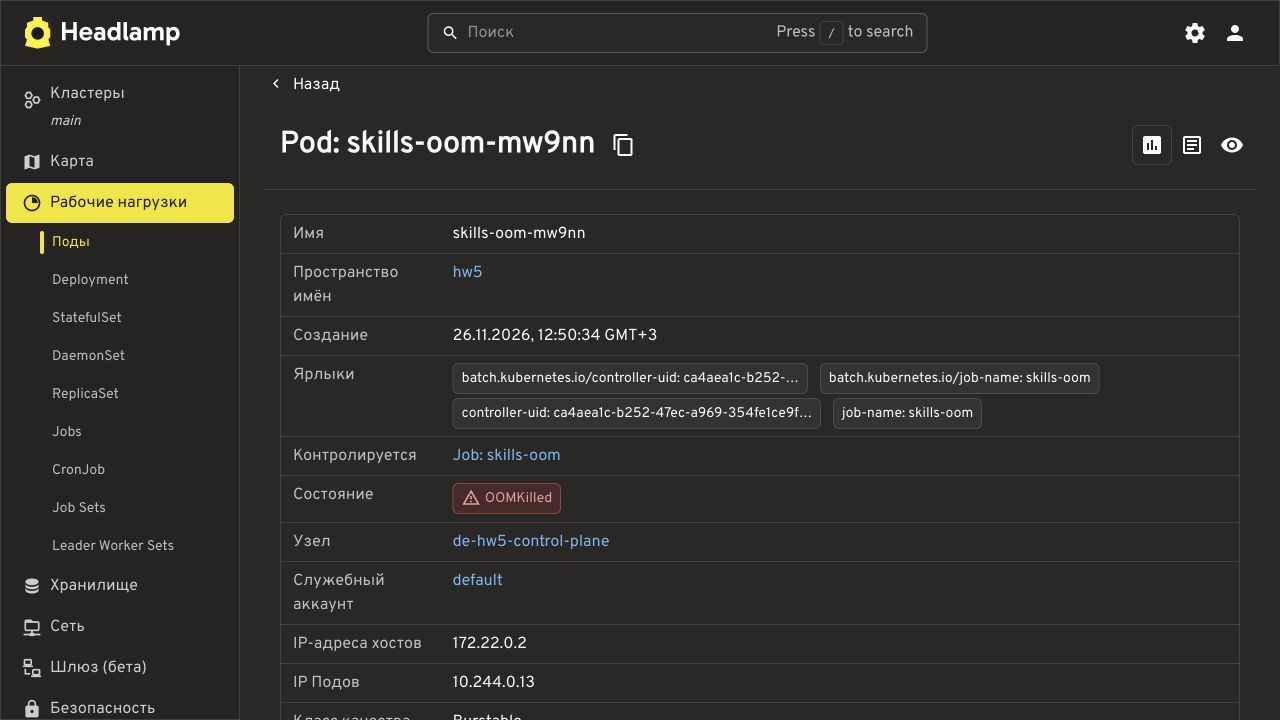
\includegraphics[width=\linewidth]{images/03-headlamp-oom.png}
\par\smallskip{\footnotesize Рис. 3. В Headlamp сохранённый Pod имеет состояние OOMKilled.}
\end{center}

\clearpage
\section*{Параллельный запуск в Headlamp}
\begin{center}
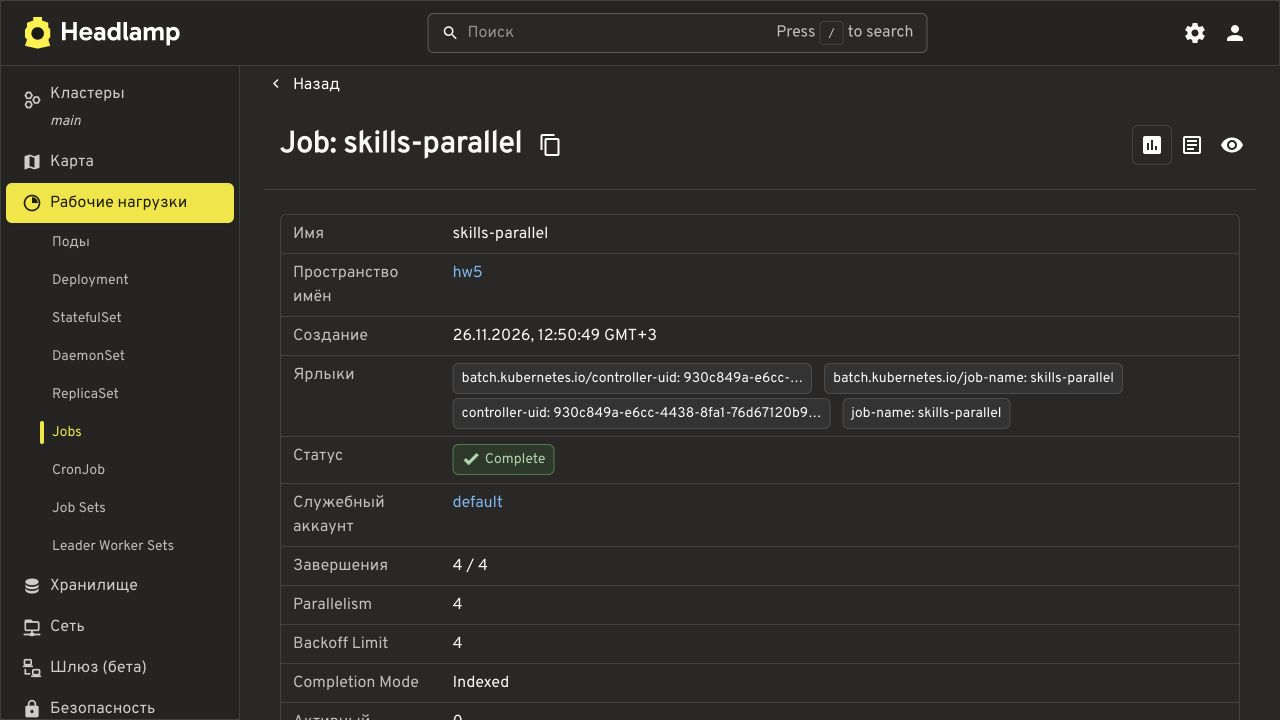
\includegraphics[width=\linewidth]{images/04-headlamp-parallel.png}
\par\smallskip{\footnotesize Рис. 4. Indexed Job завершён: Complete, 4/4, parallelism=4.}
\end{center}
\begin{center}
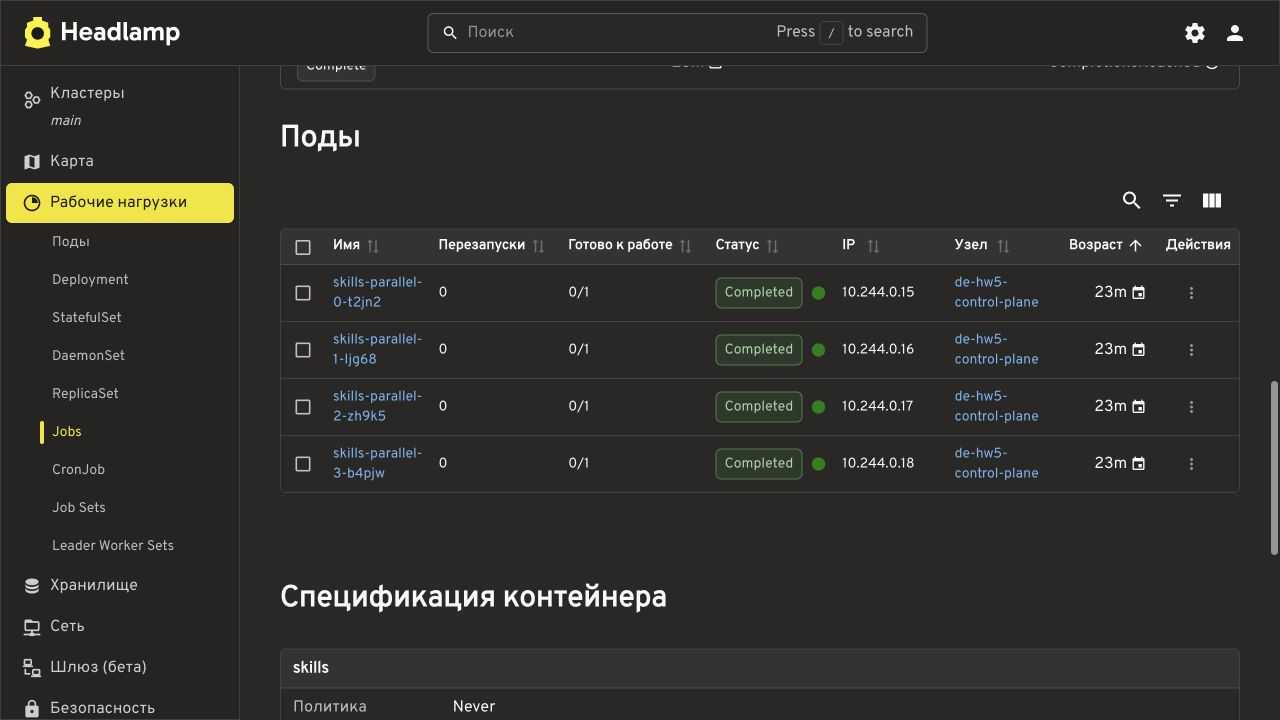
\includegraphics[width=\linewidth]{images/05-headlamp-workers.png}
\par\smallskip{\footnotesize Рис. 5. Все четыре работника с индексами 0--3 завершились: Completed.}
\end{center}

\clearpage
\section*{Вытеснение и квота в Headlamp}
\begin{center}
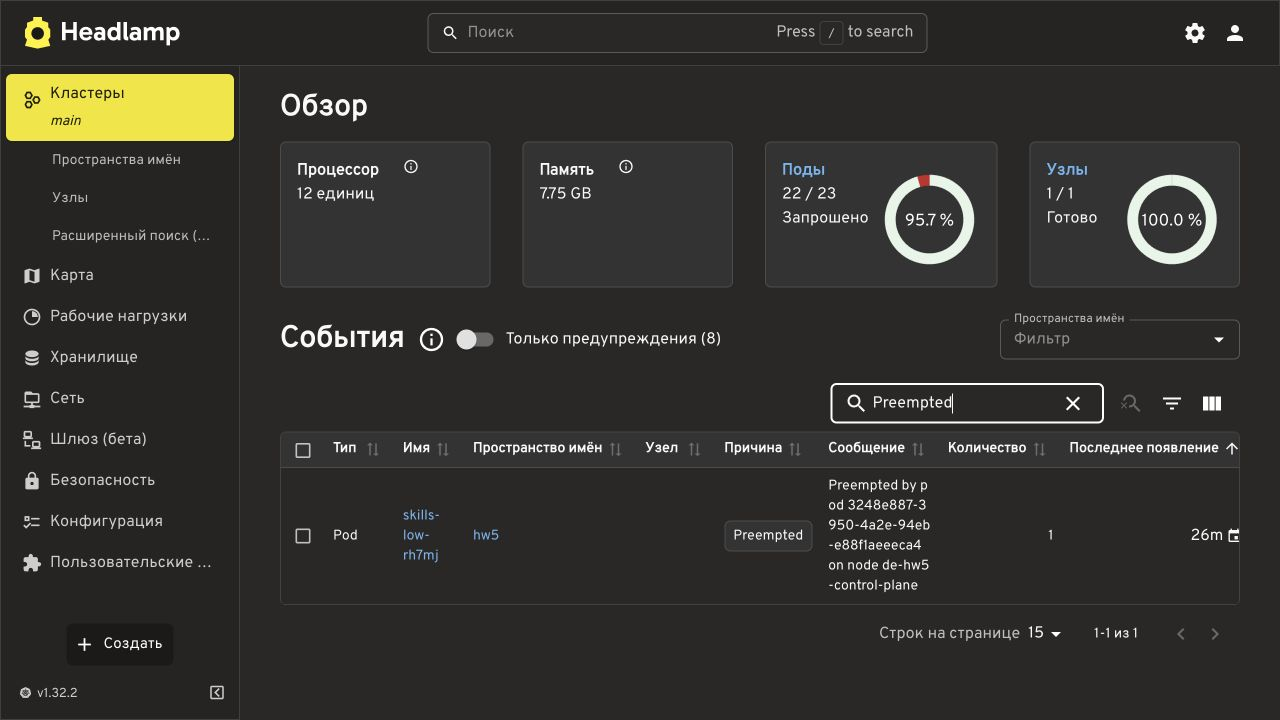
\includegraphics[width=\linewidth]{images/06-headlamp-preemption.png}
\par\smallskip{\footnotesize Рис. 6. Событие Preempted у низкоприоритетного Pod skills-low.}
\end{center}
\begin{center}
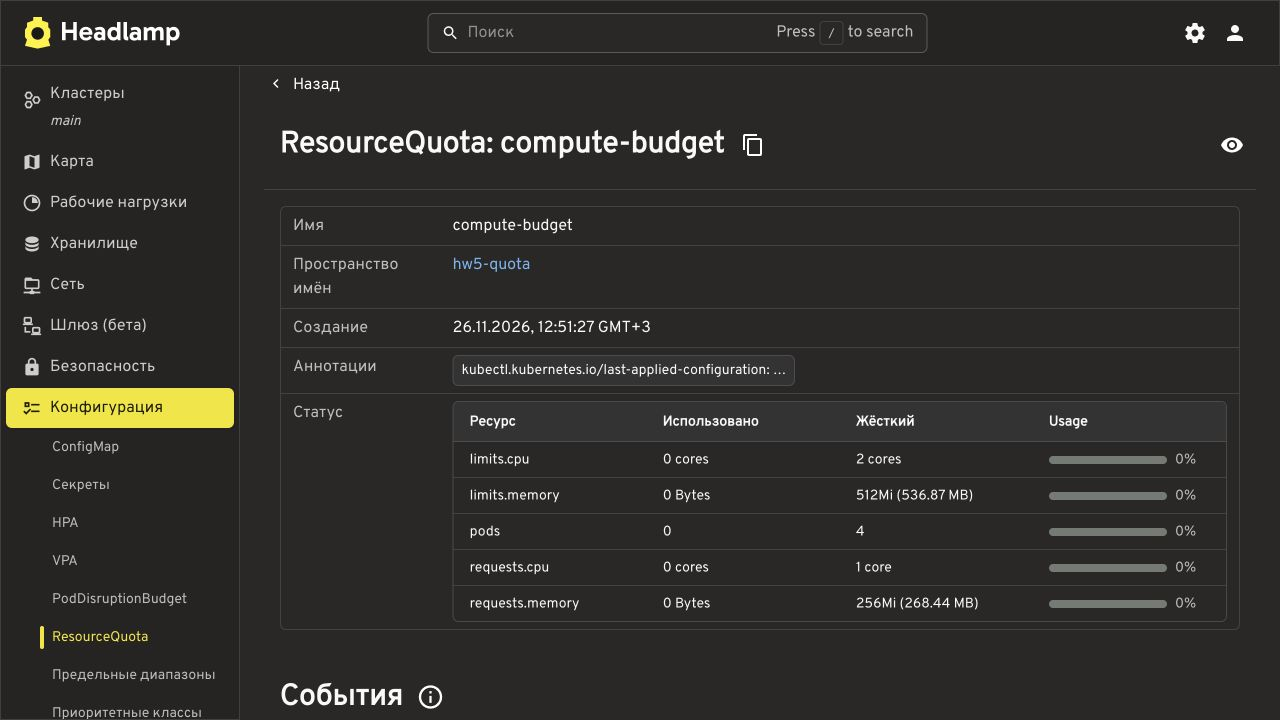
\includegraphics[width=\linewidth]{images/07-headlamp-quota.png}
\par\smallskip{\footnotesize Рис. 7. Квота compute-budget после освобождения ресурсов: запрос CPU ограничен одним ядром.}
\end{center}
\end{document}
